\section{IHM19 model (model ID: 47)}
The IHM19 model (fig.~\ref{fig:47_schematic}) was created in a master's thesis at the Institute for Hydrology and Meteorology at the Technical University of Dresden (Germany) for a small catcment in the Bavarian Forest National Park \citep{Brandes2020}. The Forellenbach basin was originally covered by a sprouce forest, when the tree population dramatically declined due to a bark beetle infestation in the 1990s and 2000s. The model was developed to test the previously identified main features of the catchment that influence the unique flood reaction with a lumped approach. One very important factor is the increase in macropores, due to root channels, which formed after 60\% of the forest cover perished.
The model aims to represent:
\begin{itemizecompact}
\item Interception;
\item Separate macropore storage;
\item Combined soil and vegetation evapotranspiration;
\item Interflow when soil moisture exceeds storage capacity;
\item Percolation to a lower soil storage with baseflow.
\end{itemizecompact}

\subsection{MARRMoT model name}
m\_46\_classic\_12p\_8s \\

% Model layout figure
\begin{figure}{}
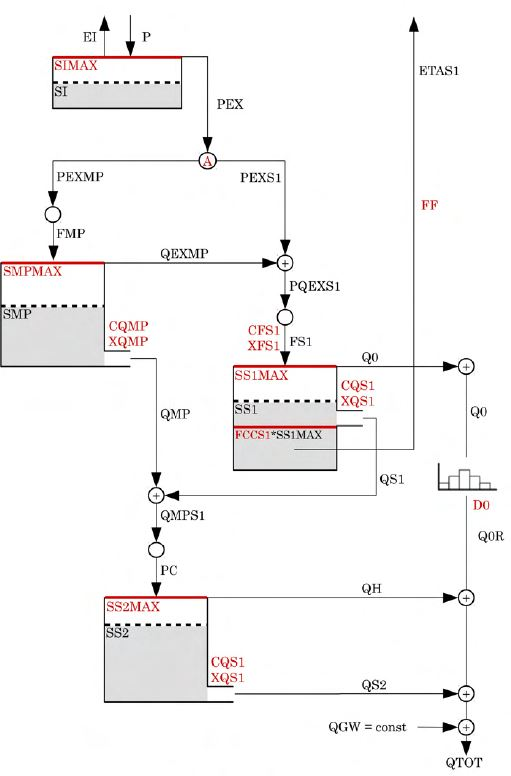
\includegraphics[width=10cm,keepaspectratio]{./AppA_files/47_schematic.jpg}
\caption{Structure of the IHM19 model} \label{fig:47_schematic}
\end{figure}

% Equations
\subsection{Model equations}

\begin{align}
	\frac{dSI}{dt} &= P-EI-PEX \\
	E_{px} &= 
	\begin{cases}
		E_p, & \text{if } SI > 0 \\
		0, & \text{otherwise}\\
	\end{cases}\\
	PEX &= 
	\begin{cases}
		P, & \text{if } SI \geq SIMAX \\
		0, & \text{otherwise}
	\end{cases}\\
	PEXMP &= (1-A)\cdot PEX\\
	PEXS1 &= A\cdot PEX
\end{align}

Where $SI$ is the current interception storage, refilled by precipitation $P$ and emptied by interception evaporation $EI$ occurring at the potential rate, when possible.
When the maximum capacity of the interception storage $SIMAX$ is exceeded throughfall $PEX$ forms and drips to the soil surface.
$PEX$ is divided into pacropore excess precipitation $PEXMP$ which forms the possible inflow into macropore storage $SMP$ and excess precipitation for the soil storage $PEXSI$.

\begin{align}
	\frac{dSMP}{dt} &= FMP-QMP \\
	FMP &= 
	\begin{cases}
		PEXMP, & \text{if } SMP < SMPMAX\\
		0, & \text{otherwise}
	\end{cases}\\[4pt]
	QMP &= CQMP\cdot SMP^{XQMP}\\[4pt]
	QEXMP &= PEXMP - FMP\\[4pt]
	PQEXS1 &= PEXS1 + QEXMP
\end{align}

Macropore storage $SMP$ is refilled by macropore infiltration $FMP$, which is equal to $PEXMP$ until maximum macropore storage $SMPMAX$ is reached.
The runoff from the macropore storage $QMP$ depends on current storage $SMP$, time-parameter $CQMP$ and scaling parameter $XQMP$.
When the macropore storage is full, macropore excess flow $QEXMP$ forms on the soil surface.
$PEXS1$ and $QEXMP$ together form the possible flow to the first soil layer $PQEXS1$.

\begin{align}
	\frac{dP=SS1}{dt} &= FS1 - ETAS1 - QS1 \\
	FS1 &=
	\begin{cases}
		CFS1 \cdot \exp \left(-XFS1\cdot\frac{SS1}{SS1MAX}\right), & \text{if } SS1 < SS1MAX\\
		0, & \text{otherwise}
	\end{cases}\\[4pt]
	ETAS1 &=
     	\begin{cases}
		FF\cdot E_p + (1-FF)\cdot\frac{SS1}{SS1MAX}\cdot E_p, & \text{if } SS1 > FCCS1\cdot SS1MAX\\
		FF\cdot\frac{SS1}{FCCS1\cdot SS1MAX}\cdot E_p + (1-FF)\cdot\frac{SS1}{SS1MAX}\cdot E_p, & \text{otherwise}
	\end{cases}\\[4pt]
	QS1 &=
	\begin{cases}
		CQS1 \cdot (SS1 - FCCS1\cdot SS1MAX)^{XQS1}, & \text{if } SS1 > FCCS1\cdot SS1MAX\\
		0, & \text{otherwise}
	\end{cases}\\[4pt] 
	Q0&=PQEXS1-FS1\\[4pt] 
	QMPS1 &= QMP + QS1
\end{align}

The upper soil storage $SS1$ is filled by soil infiltration $FS1$ and drained by soil runoff $QS1$ as well as evapotranspiration $ETAS1$.
The soil infiltration rate $FS1$ is calculated with an exponentially declining function with maximum infiltration rate $CFS1$ and a loss exponent $XFS1$, it is also dependent on the current soil storage and becomes zero as soon as $SS1$ reaches $SS1MAX$.
The runoff $QS1$ is calculated with a non-linear function, depending on a time parameter $CQS1$ and a scaling parameter $XQS1$.
It only occurs when the current soil storage $SS1$ exceeds the field capacity of soil ($FCCS1\cdot SS1MAX$).
When the current storage in $SS1$ is smaller thatn the field capacity, it is emptied only by evapotranspiration $ETAS1$.
Parameter to calculate the actual evapotranspiration are the forest fraction $FF$ (transpiration), maximum soil storage $SS1MAX$ and field capacity coefficient $FCCS1$ (evaporation).
If the soil storage of the first layer is filled and inflow still occurs through $PQEXS1$, surface runoff $Q0$ is produced.
The surface runoff is routed through a full triangular routing-fuction with a routing delay based on parameter $D0$.
The sum of the runoffs from macropore and first soil storage $QMPS1$ is the potential inflow into the lower soil store $SS2$.

\begin{align}
	\frac{dSS2}{dt} &= PC-QS2 \\
	PC &= 
	\begin{cases}
		QMPS1, & \text{if } SS2 < SS2MAX \\
		0, & \text{otherwise}\\
	\end{cases}\\[4pt]
	QS2 &= CQS2\cdot SS2^{XQS2}\\[4pt]
	QH &= QMPS1 - PC\\[4pt]
	QTOT &= Q0R + QH + QS2
\end{align}

The second soil layer $SS2$ is filled by percolation $PC$, which is equal to the runoff from the uppr soil store $QSMPS1$, as long as the second soil layer is not saturated.
If $SS2MAX$ is reached and there is still runoff from above, interflow $QH$ is produced between the soil layers.
The runoff from the second soil layer $QS2$ is the baseflow of the model and is calculated similarly to the macropore-runoff, with a non-linear function and two parameters for time and scaling $CQS2$ and $XQS2$.
The total runoff $QTOT$ is calculated by summing the routed surface runoff $Q0R$, interflow $QH$ and baseflow $QS2$.

\subsection{Parameter overview}
% Table generated by Excel2LaTeX from sheet 'Sheet1'
\begin{table}[htbp]
  \centering
    \begin{tabular}{lll}
    \toprule
    Parameter & Unit  & Description \\
    \midrule
    $SIMAX$ & $mm$   & Maximum interception storage \\
    $A$ & $-$   & Splitting coefficient for excess precipitation \\
    $FF$ & $-$  & Forest fraction \\
    $SMPMAX$ & $mm$ & Maximum macropore storage \\
    $CQMP$ & $d^{-1}$   & Runoff time parameter for macropore store \\
    $XQMP$ & $-$   & Runoff scale parameter for first macropore store \\
    $SS1MAX$ & $mm$   & Maximum soil moisture storage in first soil layer\\
    $FCCS1$ & $-$  & Field capacity coefficient of first soil layer \\
    $CFS1$ & $mm\cdot d^{-1}$   & Maximum infiltration rate of first soil layer \\
    $XFS1$ & $-$ & Infiltration loss exponent of first soil layer \\
    $CQS1$ & $d^{-1}$ & Runoff time parameter for first soil layer \\
    $XQS1$ & $-$ &  Runoff scale parameter for first soil layer\\
    $SS2MAX$ & $mm$ &  Maximum soil moisture storage in second soil layer\\
    $CQS2$ & $d^{-1}$ & Runoff time parameter for second soil layer \\
    $XQS2$ & $-$ &  Runoff scale parameter for second soil layer \\
    $D0$ & $d$ & Surface runoff flow delay \\
    \bottomrule
    \end{tabular}%
  \label{tab:addlabel}%
\end{table}%
